\documentclass{scrreprt}
\usepackage[utf8]{inputenc}
\usepackage{listings}
\lstset{
  basicstyle=\fontsize{10}{8}
}
\usepackage{graphicx}
\usepackage{hyperref}
\usepackage{float}
\pretolerance=10000

% place images on empty pages at the top
% see http://tex.stackexchange.com/questions/66252/placing-the-figure-exactly-at-the-top-of-the-page-in-latex
\makeatletter
\setlength{\@fptop}{0pt}
\makeatother


\begin{document}
\graphicspath{{images/}}

\author{
Michael Srocka \\
\texttt{srocka@greendelta.com}
}

\title{openLCA Developer Guide}

\maketitle

\chapter{Introduction}
openLCA\footnote{\url{http://openlca.org}} is a free, professional Life Cycle Assessment (LCA) and footprint software.  It is an open-source software and licensed under the Mozilla Public License version 2.0\footnote{\url{http://www.mozilla.org/MPL/2.0/}}. Thus, the software is fully transparent and can be modified by anyone. Additionally, it is possible to add new functionality to openLCA via plugins. This guide explains how you can set up a development environment to build openLCA from source and explains the general structure of the openLCA source code. It also shows in a small example how you can develop an openLCA plugin.

The picture below shows the overall architecture of openLCA. It is a Java application that runs on the Eclipse Rich Client Platform (RCP)\footnote{\url{http://wiki.eclipse.org/Rich_Client_Platform}}. However, the core functionality is independent from the Eclipse runtime and can be integrated in every other application that runs on the Java Virtual Machine (JVM). This core functionality is bundled in a project called \texttt{olca-modules} (the openLCA modules) whereas the project name of openLCA application is \texttt{olca-app} (the openLCA application).    

\begin{figure}[H]
\centering
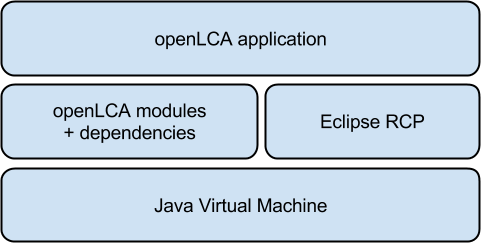
\includegraphics[width=0.7\textwidth]{images/openlca_structure.png}
\caption{Structure of openLCA}
\end{figure} 

The official source code repository of the \texttt{olca-modules} project is \url{https://github.com/GreenDelta/olca-modules} and for the \texttt{olca-app} project it is \url{https://github.com/GreenDelta/olca-app}. 


\chapter{Setting up a development environment}

\section{Java}
As openLCA is a Java application, the first thing you should install is the Java Development Kit (JDK). The openLCA application uses features of Java 8 and therefore you need the JDK 8 to build the application. If you just want to build the openLCA modules the JDK 7 should be sufficient. We recommend to use Oracle Java\footnote{\url{http://www.oracle.com/technetwork/java/javase/downloads/index.html}} but it should also work with Open JDK\footnote{\url{http://openjdk.java.net/}}. For Windows and Mac OS X you can just use the installers provided on the Oracle download site. For Linux the best procedure is probably the one described here: \url{ http://askubuntu.com/questions/56104/how-can-i-install-sun-oracles-proprietary-java-jdk-6-7-8-or-jre}. 

\section{Manage the source code via Git}
The source code of openLCA is managed via Git\footnote{\url{http://git-scm.com/}} and hosted on Github\footnote{\url{http://github.com/}}. You can find the source repository of the openLCA modules under \url{https://github.com/GreenDelta/olca-modules} and the repository of the openLCA application under https://github.com/GreenDelta/olca-app. The easiest way to get the code and to stay up to date with the development of openLCA is to install git and clone these repositories:

\begin{lstlisting}[language=bash]
git clone https://github.com/GreenDelta/olca-app
git clone https://github.com/GreenDelta/olca-modules
\end{lstlisting} 

This will create the two folders \texttt{olca-app} and \texttt{olca-modules} in the current directory which contain the complete source code.

\section{Maven and missing dependencies}
We use Maven\footnote{\url{http://maven.apache.org/}} to manage the build and the dependencies of the openLCA modules and for the dependency management in the openLCA application. Thus, you need to have Maven installed. 
The \texttt{olca-modules} is a Maven multi-modules project. If you navigate to this repository and type

\begin{lstlisting}[language=bash]
mvn install -DskipTests=true
\end{lstlisting}    

Maven will try to build and install all the sub-modules of this project into your local repository. If you do this the first time the build will probably fail because we need ojAlgo\footnote{\url{http://ojalgo.org//}} which is unfortunately not managed via the central Maven repository. Thus, we need to download ojAlgo and install it into our local repository manually. Therefore, download the current ojAlgo package and install the \texttt{ojalgo-VERSION.jar} using the following command:

\begin{lstlisting}[language=bash]
mvn install:install-file -Dfile=ojalgo-VERSION.jar \ 
-DgroupId=org.ojalgo -DartifactId=ojalgo \
-Dversion=VERSION -Dpackaging=jar
\end{lstlisting}

You may also have to change the version in the dependency declaration in the file \texttt{olca-modules/olca-core/pom.xml}:

\begin{lstlisting}
<dependency>
  <groupId>org.ojalgo</groupId>
  <artifactId>ojalgo</artifactId>
  <version>VERSION</version>
</dependency>
\end{lstlisting} 

If you run the install command again everything should work now. \footnote{Note if you run the comment without the \texttt{-DskipTests=true} flag the build will only work if you have the native libraries in the \texttt{olca-eigen} module correctly installed as this is required to pass the tests (this is described later).} Now we need to copy our openLCA modules libraries and all the other dependencies into the openLCA application project. We also use a Maven script for this task which is located under \texttt{olca-app/olca-app/pom.xml}. To make the development cycle a bit more convenient there is a small shell/batch script located in the \texttt{olca-app} project which combines all the Maven related tasks:

\begin{lstlisting}[language=bash]
 # compile and install olca-modules and update 
 # the dependencies in olca-app
 ./olca-app/update_modules.sh
\end{lstlisting}	   

\section{Eclipse}
The \texttt{olca-modules} and \texttt{olca-app} projects are already configured as Eclipse projects. Thus, you can directly import them into an Eclipse project. Select the folder where your code repositories are located and you can import these projects like in the following picture:

\begin{figure}[H]
\centering
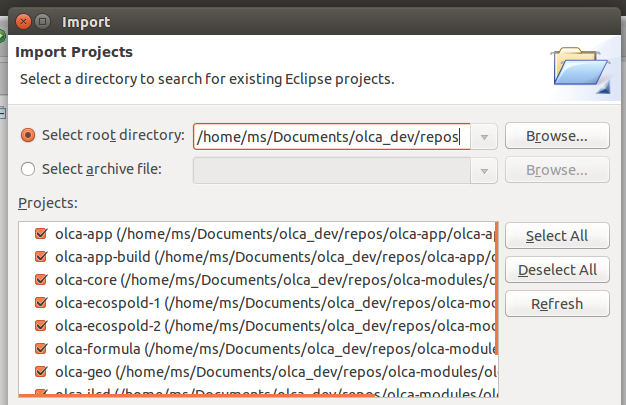
\includegraphics[width=0.9\textwidth]{images/eclipse_import_projects.png}
\caption{Import existing projects into an Eclipse workspace}
\end{figure} 

After the import you will see again a lot of errors which we will fix in the following. First, install the Maven integration for Eclipse from the Eclipse Marketplace (Help/Marketplace): 

\begin{figure}[H]
\centering
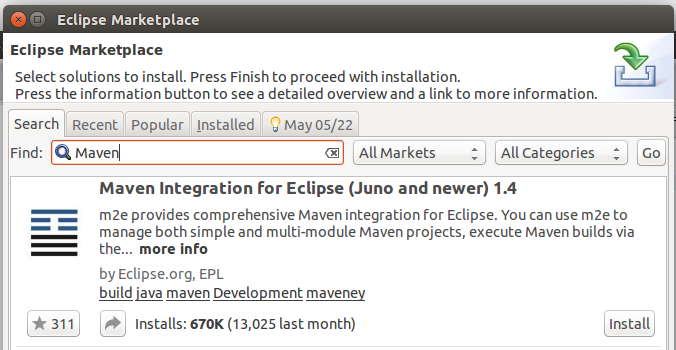
\includegraphics[width=0.9\textwidth]{images/eclipse_maven_integration.png}
\caption{Install the Eclipse Maven plugin}
\end{figure}  

Then, download the runtime project from \url{ https://drive.google.com/file/d/0Bw9cXD8IWJzzRERLLVNXU19oNGM/edit?usp=sharing} and import it as existing project into the workspace (chose 'Select archive file'):

\begin{figure}[H]
\centering
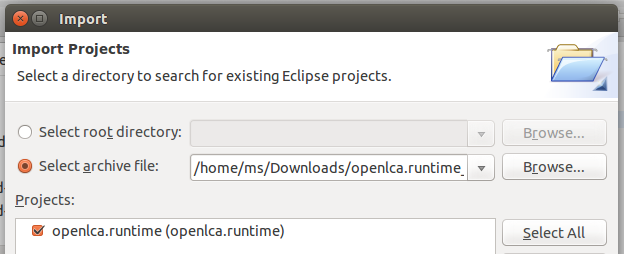
\includegraphics[width=0.9\textwidth]{images/eclipse_import_runtime.png}
\caption{Import the runtime project}
\end{figure}  

Open the file \texttt{platform.target} in the runtime project and click the option \texttt{Set as target platform} in the target definition editor.

Finally, set the JDK 8 as the default Java runtime under Preferences/Java/Installed JREs and the compiler compliance level to 1.8 under Preferences/Java/Compiler.

\chapter{Project structure and development cycle}

\section{Project structure}
When you set up your development environment as described above you should see the following projects in the Eclipse workspace:

\begin{figure}[H]
\centering
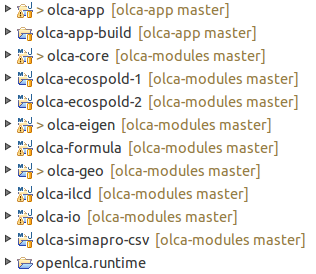
\includegraphics[height=200px]{images/structure_projects.png}
\caption{openLCA projects}
\end{figure} 

\begin{description}
  \item[olca-app] \hfill \\
  Contains the openLCA application that is based on Eclipse RCP: the user interface, editor logic, database management etc.
   
  \item[olca-app-build] \hfill \\
  Contains the build scripts, tools, and runtimes for compiling and packaging the RCP application for Windows, Linux, and Mac OS.
  
  \item[olca-core] \hfill \\
  Contains the openLCA data model, calculation procedures, and functionality for interacting with a database.
  
  \item[olca-ecospold-1] \hfill \\
  Contains the data model for automatic binding of EcoSpold 1 XML files to object graphs and the other way around.
  
  \item[olca-ecospold-2] \hfill \\
  Same as olca-ecospold-1 but for the EcoSpold 2 data format.
  
  \item[olca-eigen] \hfill \\
  Provides JNI\footnote{\url{http://docs.oracle.com/javase/8/docs/technotes/guides/jni/}} wrappers to the high performance math libraries OpenBLAS\footnote{\url{http://www.openblas.net/}} and Eigen\footnote{\url{http://eigen.tuxfamily.org}}.
  
  \item[olca-formula] \hfill \\
  Contains a formula interpreter that is used for parameter evaluation in different scopes in openLCA. 
  
  \item[olca-geo] \hfill \\
  Contains the functionality for localized LCIA calculations including the handling of shapefiles and KML data.
  
  \item[olca-ilcd] \hfill \\
  Contains the data model for automatic binding of ILCD XML files to object graphs and the other way around. It supports the storing and reading of ILCD files from folders, ZIP files, and ILCD network nodes (i.e. soda4LCA servers\footnote{\url{http://www.iai.kit.edu/www-extern/index.php?id=soda4lca&L=1}}).
  
  \item[olca-io] \hfill \\
  Contains the mappings and export/import interfaces from the openLCA data model to various data formats.
  
  \item[olca-simapro-csv] \hfill \\
  Contains a parser and data model for reading SimaPro CSV files.
  
  \item[openlca.runtime] \hfill \\
  Contains the dependencies (i.e. the OSGi bundles) of the openLCA RCP application.
  
\end{description}

Each project should also have a README file in its root folder which explains the content and structure of the respective project in more detail.

\section{The development cycle}
As the olca-app and olca-modules project are independent from each other, the modules have to be updated in the olca-app project when they changed. We use Maven (as described above) to automate these updates. Just run the \texttt{update\_modules.bat/sh} script when you changed something in the olca-modules and it will build the modules, install them in your local Maven repository, and update them in your olca-app project. 

\section{Make the tests running}
The openLCA modules projects contain quite some unit tests which you can run with the standard Maven test command or via the user interface of your Java IDE. When you download the source code repository these tests will initially fail because of the missing native libraries in the olca-eigen module. You can fix this by either compiling the native libraries by yourself or copying the prepared builds into the olca-eigen project following the instructions in this READEME file: \url{https://github.com/GreenDelta/olca-modules/tree/master/olca-eigen}. The folder structure of the olca-eigen project should look like this (you only need the library for your operating system):

\begin{figure}[H]
\centering
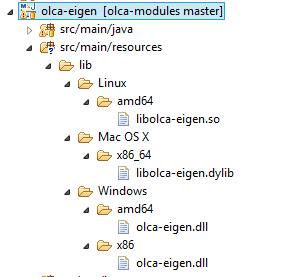
\includegraphics[height=200px]{images/structure_native_libs.png}
\caption{Folder structure in olca-eigen}
\end{figure}  


\chapter{Plugin development}
Because the openLCA application is based on the Eclipse Rich Client Platform we can use the Eclipse plugin features also in openLCA. With this it is possible to develop and distribute additional functionalities as add-ons/plugins. In the following the development of a plugin is described on a practical exampled. It is assumed that the development environment is already set up as described above. This project is open source\footnote{\url{https://github.com/msrocka/xolca-app-gexf}} and you can use it as a template for the development of other openLCA plugins.

\section{The example: an GEXF export of product systems}
In the following we will develop a plugin for the export of product system graphs as GEXF files. GEXF stands for Graph Exchange XML Format\footnote{\url{http://gexf.net}} which is an open format for exchanging graphs and networks. We will develop a simple but nice export so that we can open and visualize a product system graph in Gephi\footnote{\url{https://gephi.org}}.  

\section{Create the plugin}
We create a new plugin \texttt{xolca-app-gefx} and keep the settings in the wizard (except for the package names which we make a bit more Java friendly):

\begin{figure}[H]
\centering
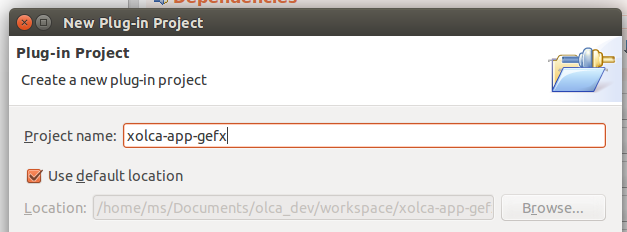
\includegraphics[width=0.9\textwidth]{images/plugin_create.png}
\caption{Create the plugin}
\end{figure}  

After this the new plugin project looks like this:

\begin{figure}[H]
\centering
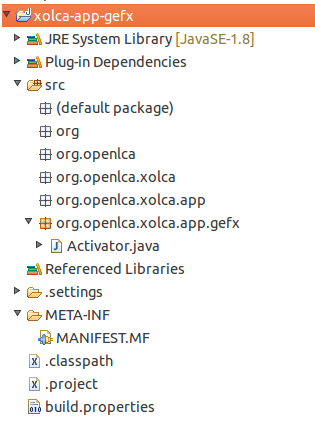
\includegraphics[height=200px]{images/plugin_initial_project.png}
\caption{The initial project layout}
\end{figure}  

Now we copy the product configuration \texttt{openLCA.product} from the \texttt{olca-app} project into the plugin project and rename it, e.g. \texttt{gefx\_export.product}. Then we open the product configuration and add our plugin in the dependency tab:

\begin{figure}[H]
\centering
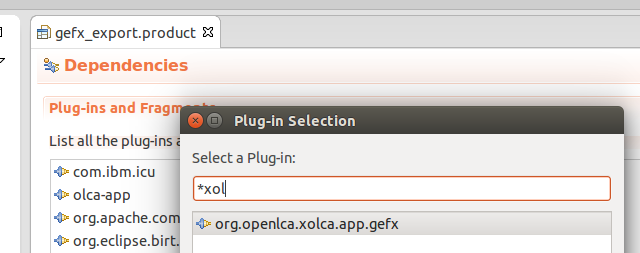
\includegraphics[width=0.9\textwidth]{images/plugin_product_config.png}
\caption{Add the plugin to the product configuration}
\end{figure}   

When we now run this configuration our plugin is loaded and we can test its functionality. 

(TODO: picture: plugin in configuration details; Java 8 entry in manifest may results in a problem - fixed in Eclipse 4.4?)

Finally, we add the \texttt{olca-app} bundle to the plugin dependencies so that we can use the openLCA API. Therefore open the \texttt{MANIFEST.MF} and add the \texttt{olca-app} entry:

\begin{figure}[H]
\centering
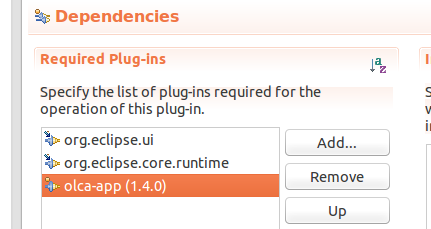
\includegraphics[height=150px]{images/plugin_add_app_dependency.png}
\caption{Add the olca-app bundle to the plugin dependencies}
\end{figure}  

\section{Adding the export wizard}
We now write the export wizard:

\begin{lstlisting}[language=Java]
public class ExportWizard extends Wizard implements IExportWizard{
  
  private ModelSelectionPage page;
	
  @Override
  public void init(IWorkbench workbench, 
    IStructuredSelection selection) {
    setWindowTitle("Export product system as GEXF file");
    setNeedsProgressMonitor(true);
  }

  @Override
  public void addPages() {
    page = new ModelSelectionPage(ModelType.PRODUCT_SYSTEM);
    addPage(page);
  }
	
  @Override
  public boolean performFinish() {
    File dir = page.getExportDestination();
    List<BaseDescriptor> models = page.getSelectedModels();
    if(dir == null || models.isEmpty())
      return true;
    // TODO: write export functionality
    return false;
  }
}
\end{lstlisting}

And we register the wizard in the \texttt{plugin.xml} of our project:

\begin{lstlisting}[language=xml]
<?xml version="1.0" encoding="UTF-8"?>
<?eclipse version="3.4"?>
<plugin>
 <extension
  point="org.eclipse.ui.exportWizards">
    <wizard
      class="org.openlca.xolca.app.gefx.ExportWizard"
      id="xolca-app-gefx.ExportWizard"
      name="GEXF Export">
    </wizard>
 </extension>
</plugin>
\end{lstlisting}

When we run our product configuration now the plugin should be registered in the export wizards:

\begin{figure}[H]
\centering
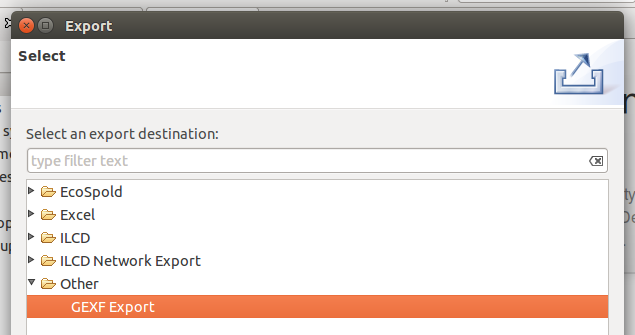
\includegraphics[width=0.9\textwidth]{images/plugin_registered.png}
\caption{Registered plugin in the export dialog}
\end{figure}  

\section{Writing the export}
The details of the export can be seen in the source code of the plugin. First we created our GEXF data model. For the XML serialization we used JAXB\footnote{\url{https://jaxb.java.net/}} and annotated our model respectively. The mapping of the product system graph to the GEXF model is done in the class \texttt{Export}. The final project structure looks like this:

\begin{figure}[H]
\centering
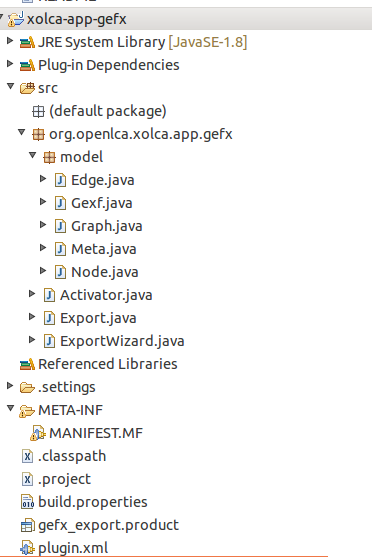
\includegraphics[height=250px]{images/plugin_final_structure.png}
\caption{Final project structure}
\end{figure}  

Finally, we call our export in the wizard:

\begin{lstlisting}[language=Java]
@Override
public boolean performFinish() {
  File dir = page.getExportDestination();
  List<BaseDescriptor> models = page.getSelectedModels();
  Export export = new Export(Database.get(), dir,
    Cache.getEntityCache());
  if (dir == null || models.isEmpty())
    return true;
  try {
    getContainer().run(true, true, (monitor) -> {
      monitor.beginTask("GEXF Export: ", models.size());
      models.forEach((d) -> {
        monitor.subTask(d.getName());
        export.doIt(d);
        monitor.worked(1);
      });
      monitor.done();
    });
    return true;
  } catch (Exception e) {
    log.error("failed to run GEXF export", e);
    return false;
  }
}
\end{lstlisting}

Now the export is fully functional and produces GEXF files that can be opened and analyzed with Gephi:

\begin{figure}[H]
\centering
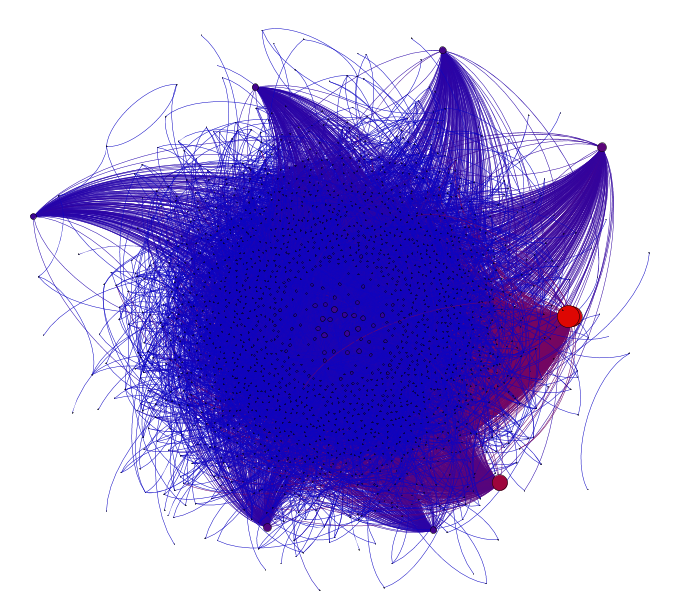
\includegraphics[width=0.9\textwidth]{images/plugin_result.png}
\caption{A product system in Gephi}
\end{figure}  

\end{document}